%!TEX root = ../main.tex

\chapter{Python}

Die Entwicklung von Python begann 1991 unter der Leitung von Guido van Rossum. Seine Ziele lagen darin, eine Sprache zu entwickeln, die einfach und intuitiv ist, deren Quelltext sich so einfach liest wie reines Englisch, die alltägliche Aufgaben mit geringer Entwicklungszeit lösen kann und Open Source sein soll.
Laut der Entwicklerumfrage von Stack Overflow wird Python jedes Jahr beliebter. 2019 überholte Python die Programmiersprache Java auf der Rangliste der beliebtesten Programmiersprachen. 

\begin{figure}[!htb]
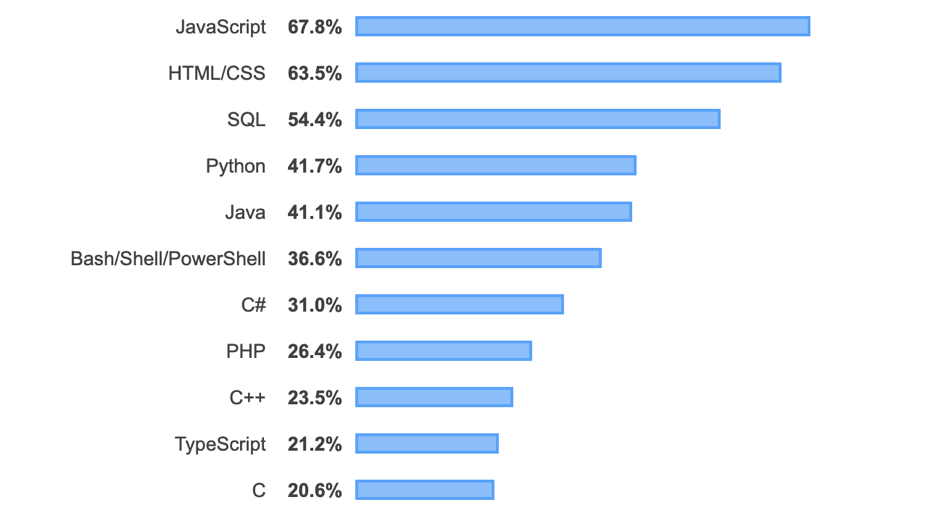
\includegraphics{stackOverflow.png}%
\caption{Rangliste der beliebtesten Programmiersprachen }
\label{img:stackoverflowBild}
\end{figure}

25\% der Entwickler, die noch nicht mit Python gearbeitet haben, möchten diese Sprache gerne lernen. Diese Lernbereitschaft wurde in den letzten drei Jahren von keiner anderen Programmiersprache überboten \cite{stackoverflow}. Das spricht sehr dafür, dass Python in den kommenden Jahren immer weiter an Bedeutung gewinnen wird. In dieser wissenschaftlichen Ausarbeitung wurde Python verwendet, um einige der Graphen und Kennlinien zu erzeugen. 

\section{Objektorientierte Programmierung in Python}

Im folgendem wird die objektorientierte Programmierung in Python anhand der vier Grundprinzipien, Generalisierung, Vererbung, Kapselung und Polymorphismus erläutert. 

\subsection{Klasse} \label{subsec:Klasse}

Zu den grundliegenden Bausteinen der objektorientierten Programmierung gehören die Klassen. Mithilfe einer Klasse lassen sich eigenen Datentypen definieren. Ein anschauliches Beispiel hierfür ist die Adresse. Die Adresse besteht aus den Strings - Straßenname und Ort und aus den integer Werten - Hausnummer und Postleitzahl. Die einzelnen Datentypen können nun in einer eigenen Klasse names Adresse gesammelt werden. Die Variablen einer Klasse bezeichnet man als Instanzvariablen. 
Instanzvariablen besitzen zugriffsrechte. Nach dem prinzip des data hiding werden private Zugriffsrechte vergeben, das bedeutet das die Instanzvariablen nur innerhalb der Klasse bekannt sind und beeinflusst werden können.
Neben Instanzvariablen können Klassen auch Methoden besitzten. Methoden können die Instanzvariablen auslesen und beeinflussen. Grundlegende Methoden sind zum Beispiel \texttt{getter} und \texttt{setter}. Werden diese Methoden implementiert, können die privaten Zugriffsrechte umgangen werden. Durch die \texttt{setter} Methoden erhält man Schreibrechte und durch die \texttt{getter} Methoden Leserechte \cite{JavaRatz}.
Instanzvariablen, Zugriffsrechte und Methoden einer Klasse lassen sich anschaulich in einem UML Klassendiagrammen darstellen. In Abbildung \ref{img:AdresseUML} ist das UML Klassendiagramm der Klasse Adresse mit seinen \texttt{getter} und \texttt{setter} Methoden und Instanzvariablen dargestellt. 

\begin{figure}[!htb]
    \centering
    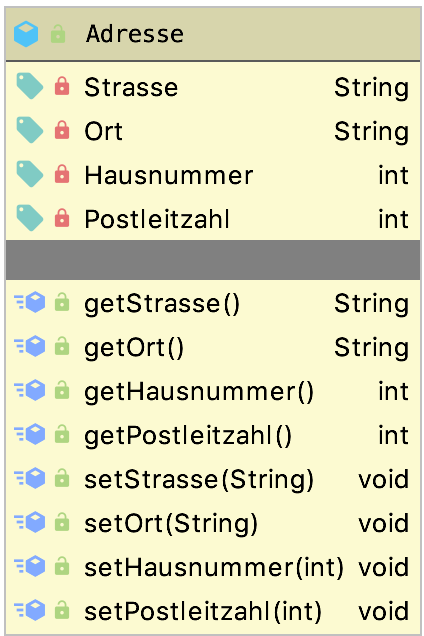
\includegraphics[scale=0.5]{AdresseUML.png}
    \caption{Die Klasse Adresse mit getter und setter Methoden}
    \label{img:AdresseUML}
\end{figure}

Um den neu definierten Datentyp zu nutzen, erzeugen wir Objekte der Klasse. Wir weisen dafür den Instanzvariablen konkrete Werte zu. Sowohl in Java als auch in Python nutzt man für die Instanziierung von Objekten eine Methode, die Konstruktor \footnote{In Python  Initialisierungsmethode} genannt wird . Der Konstruktor ist vergleichbar mit der \texttt{set} Methode. Beim aufrufen des Konstruktors übergibt man ihm die konkreten Werte der Instanzvariablen und erhält als rückgabewert eine Referenz auf das erzeugte Objekt. Die folgenden Codebeispiele zeigen die Implementierung der Klasse Adresse in Java \ref{Adressejava} und Python \ref{AdressePython}.

%Code Beispiele für die Klasse Adresse in Java und Python.
\begin{lstlisting}[caption=Die Klasse Adresse in Java, label=Adressejava]
public class Adresse
{
    //Instanzvariablen
    private String Strasse;
    private String Ort;
    private int Hausnummer;
    private int Postleitzahl;

    //Konstruktor
    public Adresse(String strasse, String ort, int hausnummer, int postleitzahl)
    {
        this.Strasse = strasse;
        this.Ort = ort;
        this.Hausnummer = hausnummer;
        this.Postleitzahl = postleitzahl;
    }

    //get Methode
    public String getStrasse() 
    {
        return Strasse;
    }

    //set Methode
    public void setStrasse (String strasse)
    {
        this.Strasse = strasse;
    }
}
\end{lstlisting}

\begin{lstlisting}[caption=Die Klasse Adresse in Python, label=lst:AdressePython,language=Python]
class Adresse:
    #Initialisierungsmethode (Konstruktor)
    def __init__(self,strasse: str, hausnummer: int, postleitzahl: int, ort: str) -> None:
        self._strasse = strasse
        self._hausnummer = hausnummer
        self._postleitzahl = postleitzahl
        self._ort = ort   

    #get Methode
    def getStrasse(self) -> str:
        return self._strasse

    #set Methode
    def setStrasse(self, strasse: str) -> None:
        self._strasse = strasse

\end{lstlisting}

Der wohl auffälligste Unterschied bei der Implementierung der Klasse \texttt{Adresse} liegt bei den Instanzvariablen. In Java werden die Instanzvariablen einzeln mit ihren Zugriffsrechten und Datentypen angegeben. Für Python wird das nicht benötigt. Die Zugriffsrechte der Instanzvariablen von Python werden nicht durch Schlüsselwörter wie \texttt{private} festgelegt, sondern durch einen Unterstrich. Hierbei handelt es sich um eine Namenskonvention. Der Unterstrich vor dem Namen der Variable signalisiert, das diese Instanzvariable als privat betrachtet werden soll. Sie hindert aber nicht daran auf die Variable zu zugreifen und zu verändern. In Python gilt die Philosophie, das der direkte Zugriff auf Attribute erlaubt und gewünscht ist \cite{PythonKalista}. Desweiteren ist die Datentyp Annotation des Rückgabewertes \footnote{def Methodenname() \textbf{\texttt{-> str}}} und der Methodenparameter in Python optional \cite{PythonBarry}. Die Initialisierung von einem konkreten Objekt der Klasse Adresse ähnelt sich in beiden Sprachen sehr, siehe Listings \ref{Konstruktor Java}, \ref{ObjektinitialisierungPython}, wobei auch hier Python mit weniger Code auskommt. 

\begin{lstlisting}[caption=Objektinitialisierung in Java, label=Konstruktor Java]
//Objektinitialisierung in Java
Adresse meineAdresse = new Adresse("Schlossstr","Berlin",01,12345);
\end{lstlisting}

\begin{lstlisting}[caption= Objektinitialisierung in Python, label=ObjektinitialisierungPython,language=Python]
#Objektinitialisierung in Python
meineAdresse = Adresse("Schlossstr","Berlin",01,12345)
\end{lstlisting}

\subsection{Generalisierung} \label{subsec:Generalisierung}

Aufbauend auf dem Kapitel Klasse \ref{subsec:Klasse} betrachten wir nun den ersten Grundpfeiler der objektorientierten Programmierung, die Generalisierung. Von Generalisierung ist dann die Rede, wenn mehrere Klassen die selben Eigenschaften teilen. Würde man die Klasse \texttt{Bus} und die Klasse \texttt{Auto} implementiert, so würden beide Klassen die Eigenschaft fahren besitzten. Gemeinsamme Eigenschaften werden in einer \textbf{Superklasse} zusammengeführt. Die Superklasse von \texttt{Bus} und \texttt{Auto} könnte die Klasse \texttt{Fahrzeug} sein. Die Klasse \texttt{Auto} kann durch die \textbf{Subklassen} \texttt{Cabrio}, \texttt{Limousine} und \texttt{Coupe} spezialisiert werden. Im Kapitel Vererbung \ref{subsec:Vererbung} wird erläutert, warum der daraus entstehende Hierarchibaum den Programmieraufwand minimiert. 


\subsection{Vererbung} \label{subsec:Vererbung}

Der im Kapitel \ref{subsec:Generalisierung} beschriebene Hierarchiebaum hat folgende Form (Abbildung. \ref{img:Hierarchiebaum}). Die Klassen \texttt{Auto}, \texttt{Bus}, \texttt{Limousine}, \texttt{Coupe} und \texttt{Cabrio} besitzten keine Instanzvariablen und keine Methoden. Nur die Klasse \texttt{Fahrzeug} implementiert die Methode \texttt{fahren()}.
Durch Vererbung sind alle Subklassen von Fahrzeug in der lage, die Methode \texttt{fahren()} aufzurufen, ohne sie einzeln zu implementieren. Der Schreibaufwand kann daher durch Vererbung minimiert werden. Vererbung hilft den Programmierer auch dabei Fehler zu vermeiden, da die Methode nur einmal implementiert und somit auch nur einmal getestet werden muss. Durch Generalisierung und Vererbung können sich Programmierer eigene Bibliotheken aus vorgefertigten Objekten  erstellen, die nur noch für die konkreten Anwendungsfälle spezialisiert werden müssen. Möchte man zum Beispiel eine neue Limousine entwickeln muss sie nur von der Klasse Limousine erben, und sie wäre bereits in der Lage zu fahren. Aus dem UML Klassendiagramm kann man ablesen, das die Klasse Fahrzeug von der Klasse \texttt{object} erbt, ohne das dies angegeben wurde. Der Grund hierfür liegt darin, das sowohl in Python als auch in Java jede Klasse von object erbt. Die Methoden, die in der Klasse object implementiert sind, können von jeder Klasse verwendet werden. Zu den Object Methoden gehören unteranderem die \texttt{equals()} Methode in Java und die \texttt{\_\_eq\_\_()} Methode in Python, mit denen man zwei Objekte auf gleichheit überprüfen kann. 

In Java wird eine Vererbung implementiert, in dem das Schlüsselwort \texttt{extends} in den Klassenkopf geschrieben wird.

\begin{lstlisting}[caption=Vererbung in Java, label=Vererbung Java]
//Die Klasse Auto erbt von der Klasse Fahrzeug
public class Auto extends Fahrzeug   
{ 
}
\end{lstlisting}

In der Sprache Python reicht es, den Namen der Superklasse in Klammern hinter den Namen der Subklasse zu schreiben.

\begin{lstlisting}[caption= Vererbung in Python \footnote{Python lässt keine leeren Klassen zu, daher muss der befehl \texttt{pass} verwendet werden}, label=lst:Vererbungpython,language=Python]
#Die Klasse Auto erbt von der Klasse Fahrzeug    
class Auto(Fahrzeug):
    pass
\end{lstlisting}


\begin{figure}[!htb]
\centering
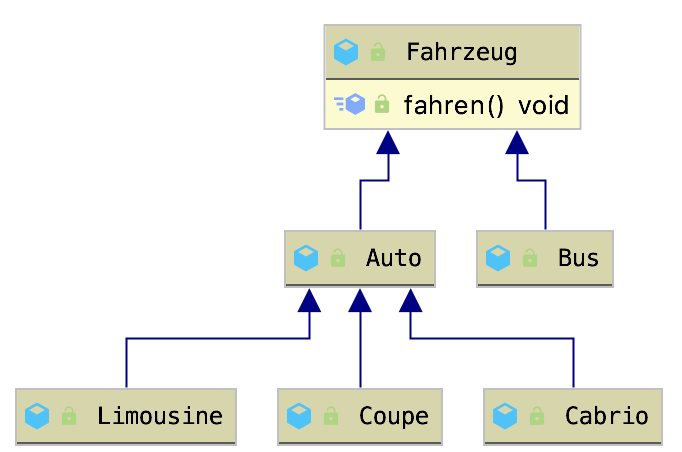
\includegraphics[scale=0.5]{FahrzeugHiera.png}%
\caption{Hierarchibaum Fahrzeug}
\label{img:Hierarchiebaum}
\end{figure}

%\subsection{Kapselung} \label{subsec:Kapselung}
%
%
\subsection{Polymorphismus} \label{subsec:Polymorphismus}
Die Klasse Object bietet neben der Vergleichsmethode auch eine Methode an um Objektinformationen in einem String zu bündeln. 
Sie wird in Java \texttt{toString()} und in Python \texttt{\_\_str\_\_()} bezeichnet. Beim Aufrufen der \texttt{\_\_str\_\_()} Methode auf ein Objekt der Klasse Auto würde der String wie folgt aussehen. 

\begin{lstlisting}[caption= \_\_str\_\_ Ausgabe Python, label=lst:strPython,language=Python]
 "__main__.Auto object at 0x7f84fb087700"   
\end{lstlisting}

Der Programmierer erhält die Information über die Klasse des Objektes und unter welcher Adresse das Objekt gespeichert ist. In Java sieht die Ausgabe ähnlich aus, mit dem Unterschied, das anstelle der Adresse, der Hashcode des Objektes ausgegeben wird. In den Meisten fällen, möchte der Programmierer jedoch Informationen über die Instanzvariablen des Objektes erhalten. Um dies zu erreichen muss die Methode überschrieben werden. Das Überschreiben der Methode wird häufig unter dem Begriff \textbf{Polymorphismus} zusammengefasst. Ein Merkmal beim überschreiben von Methoden liegt darin, das die Argumentenliste und der Rückgabetyp gleich bleibt. Um die \texttt{\_\_str\_\_()} Methode anzuwenden, fügen wir der Superklasse Fahrzeug noch einige Instanzvariablen hinzu. Die Methode \texttt{str} wird nun so überschrieben, das alle Attribute des Objektes in einem String zusammengeführt werden. In Python wird die \texttt{str} Methode automatisch aufgerufen, wenn das Object der Methode \texttt{print} übergeben wird. 

\begin{lstlisting}[caption= \_\_str\_\_ Ueberschrieben, label=lst:UeberschreibenStr,language=Python]
class Fahrzeug(object):
    def __init__(self,marke,farbe,leistung):
        self.marke = marke
        self.farbe = farbe
        self.leistung = leistung

    def fahren(self):
        print("brum  brum")



class Auto(Fahrzeug):
    def __str__(self):
        beschreibung = self.marke + "," + self.farbe + "," + str(self.leistung) + "PS"
        return beschreibung

meinAuto = Auto("Daimler","Gelb",150)
print(meinAuto)

#Ausgbae :
#Daimler,Gelb,150PS
\end{lstlisting}

